%!TEX root = Memoria_TFM.tex
\section{Databases} \label{sec:methd_databses}
In this section the databases that are used along the thesis are described in this section.\\

One database has utilized to learn \textit{Theano} and three face databases has been used in order to detect anti-spoofing. The face anti-spoofing databases have been generated with face anti-spoofing finality and has been used previously with the same purpose.\\

All the databases are formed by three subsets whose samples are not repeated among subsets:
\begin{description}[itemsep=2pt,topsep=8pt,parsep=0pt,partopsep=20pt]
\item[Training subset:] is used to train the network during epochs.
\item[Validation subset:] is used to check the performance of the network while is training. The validation subset is usually used when hyper-parameters are calculated.
\item[Test subset:] is used just at the end of the training process. The best model is chosen with regard to the best validation error. This subset should not be used until the network architecture and classifiers parameters are selected.
\end{description}

\subsection{MNIST digit database}\label{subsec:MNIST}
MNIST digit database is a image database of human written digits. This database is frequently used to learn machine learning techniques. Because of that, the database has been used, in this thesis, for learning Theano and convolutional neural networks. In addition, this database has been used in a implemented convolutional neural network (LeNet).\\
\begin{figure}[htb]
\centering
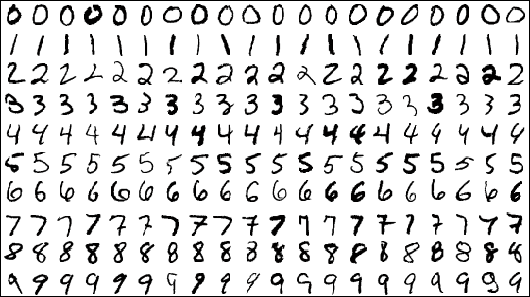
\includegraphics[width=0.6\textwidth]{images_databases/mnistExamples.png}
\caption{MNIST digit images database. Image obtained from \cite{MNISTimage}.} \label{fig:MNIST_digits}
\end{figure}
Some examples of the digit image MNIST database could be seen in \ref{fig:MNIST_digits}, image obtained from \cite{MNISTimage} and the characteristics of this database are the following ones:
\begin{itemize}[itemsep=2pt,topsep=8pt,parsep=0pt,partopsep=20pt]
 \item There are 70.000 number of unique samples.
 \item Despite of the original size of the database is 32x32 pixels, the samples of this downloaded database are 28x28 pixels in gray scale, that is 784 features per image.
 \item 10 classes could be differentiated, one per digit.
\item The samples are directly separated into train, test and validate subset.
\end{itemize}

\subsection{FRAV dataset}
FRAV database is an anti-spoofing face database built in the  \textit{FRAV} research group of the \textit{URJC University} and which is part of the Automated Border Control Gates for Europe project \cite{ABC4EU}.\\

FRAV database is formed by genuine users and spoofing attacks. Moreover, this database is formed by RGB images and NIR images, almost each RGB sample has been captured with infrared camera too.\\

Both databases are composed by genuine users samples and four distinctive attacks: printed photo, 2D mask, 2D mask with eyes cropped and real user image displayed in a tablet device.
\begin{itemize}[itemsep=2pt,topsep=8pt,parsep=0pt,partopsep=20pt]
 \item Original images of people represented in figure \ref{frav_im1-4} and figure \ref{frav_im2-5} for RBG images and figure \ref{frav_im3-5} for NIR image.
 \item Images of people printed (attack) represented in figure \ref{frav_im1-1} and figure \ref{frav_im2-1} for RBG images and figure \ref{frav_im3-1} for NIR image.
 \item Images of people with a mask (attack)represented in figure \ref{frav_im1-2}and figure \ref{frav_im2-2}for RBG images and figure \ref{frav_im3-2} for NIR image.
 \item Images of people with a mask with the eyes cropped (attack)represented in figure \ref{frav_im1-3} and figure \ref{frav_im2-3} for RBG images and figure \ref{frav_im3-3} for NIR image.
 \item Images of people in a tablet (attack)represented in figure \ref{frav_im1-4} and figure \ref{frav_im2-4} for RBG images and figure \ref{frav_im3-4} for NIR image.
 \end{itemize}

The characteristics of this database are described:
\begin{itemize}[itemsep=2pt,topsep=8pt,parsep=0pt,partopsep=20pt]
\item There are 939 people in each RGB class and 195 in each NIR class.
\item There are 2 or 5 classes: genuine class and four attacks that could be put in the same class or not.
\item Each user has a genuine image and four attacks.
\item There is one image per person.
\item Each image has its own shape.
\item The faces are centered in the image.
\item RGB images has been obtained with a professional visible light camera and NIR images with a Near infrared camera.
\item RGB images are in RGB space and NIR images are in gray-scale space.
\end{itemize}

\subsubsection{FRAV RGB database}
A representation of RGB database is shown in figure \ref{fig:RGB-frav1}, where genuine user (e) and attacks (a-d) from the same user are exposed.\\

\begin{figure}[htb]
\centering
\subfigure[printed image attack]{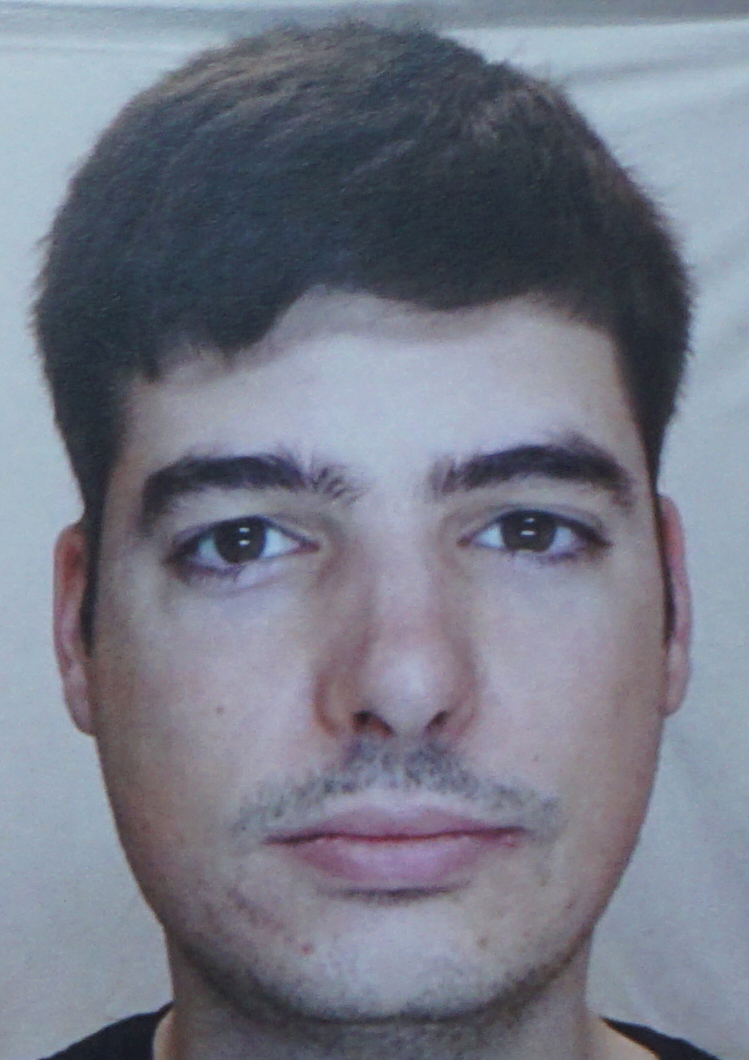
\includegraphics[width=0.18\textwidth]{images_databases/fravrgb/at1-0.JPG} \label{frav_im1-1} }
\subfigure[mask attack]{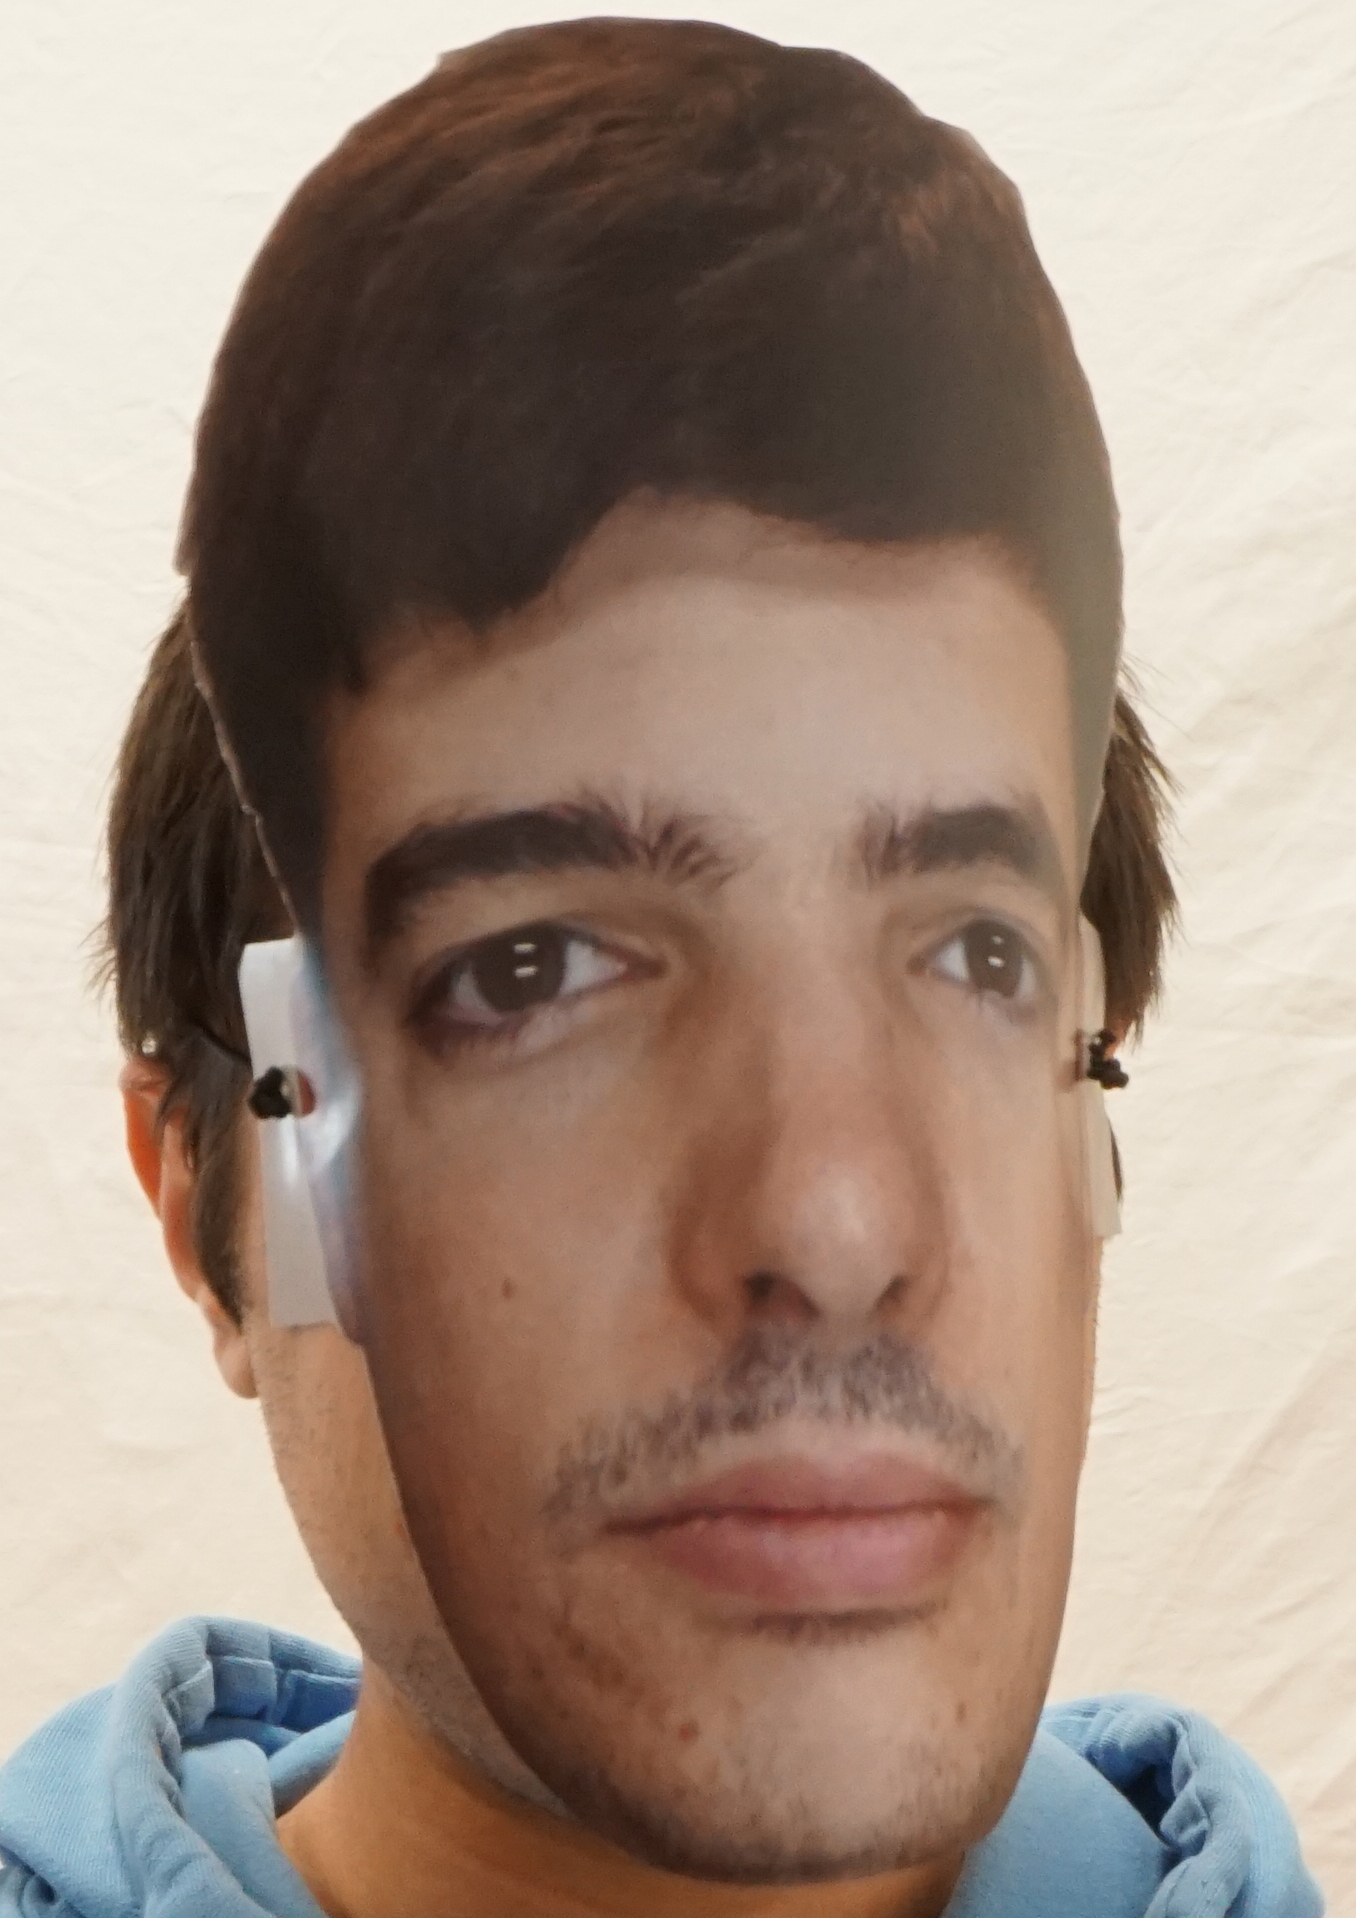
\includegraphics[width=0.18\textwidth]{images_databases/fravrgb/at2-0.JPG} \label{frav_im1-2}}
\subfigure[eye mask attack]{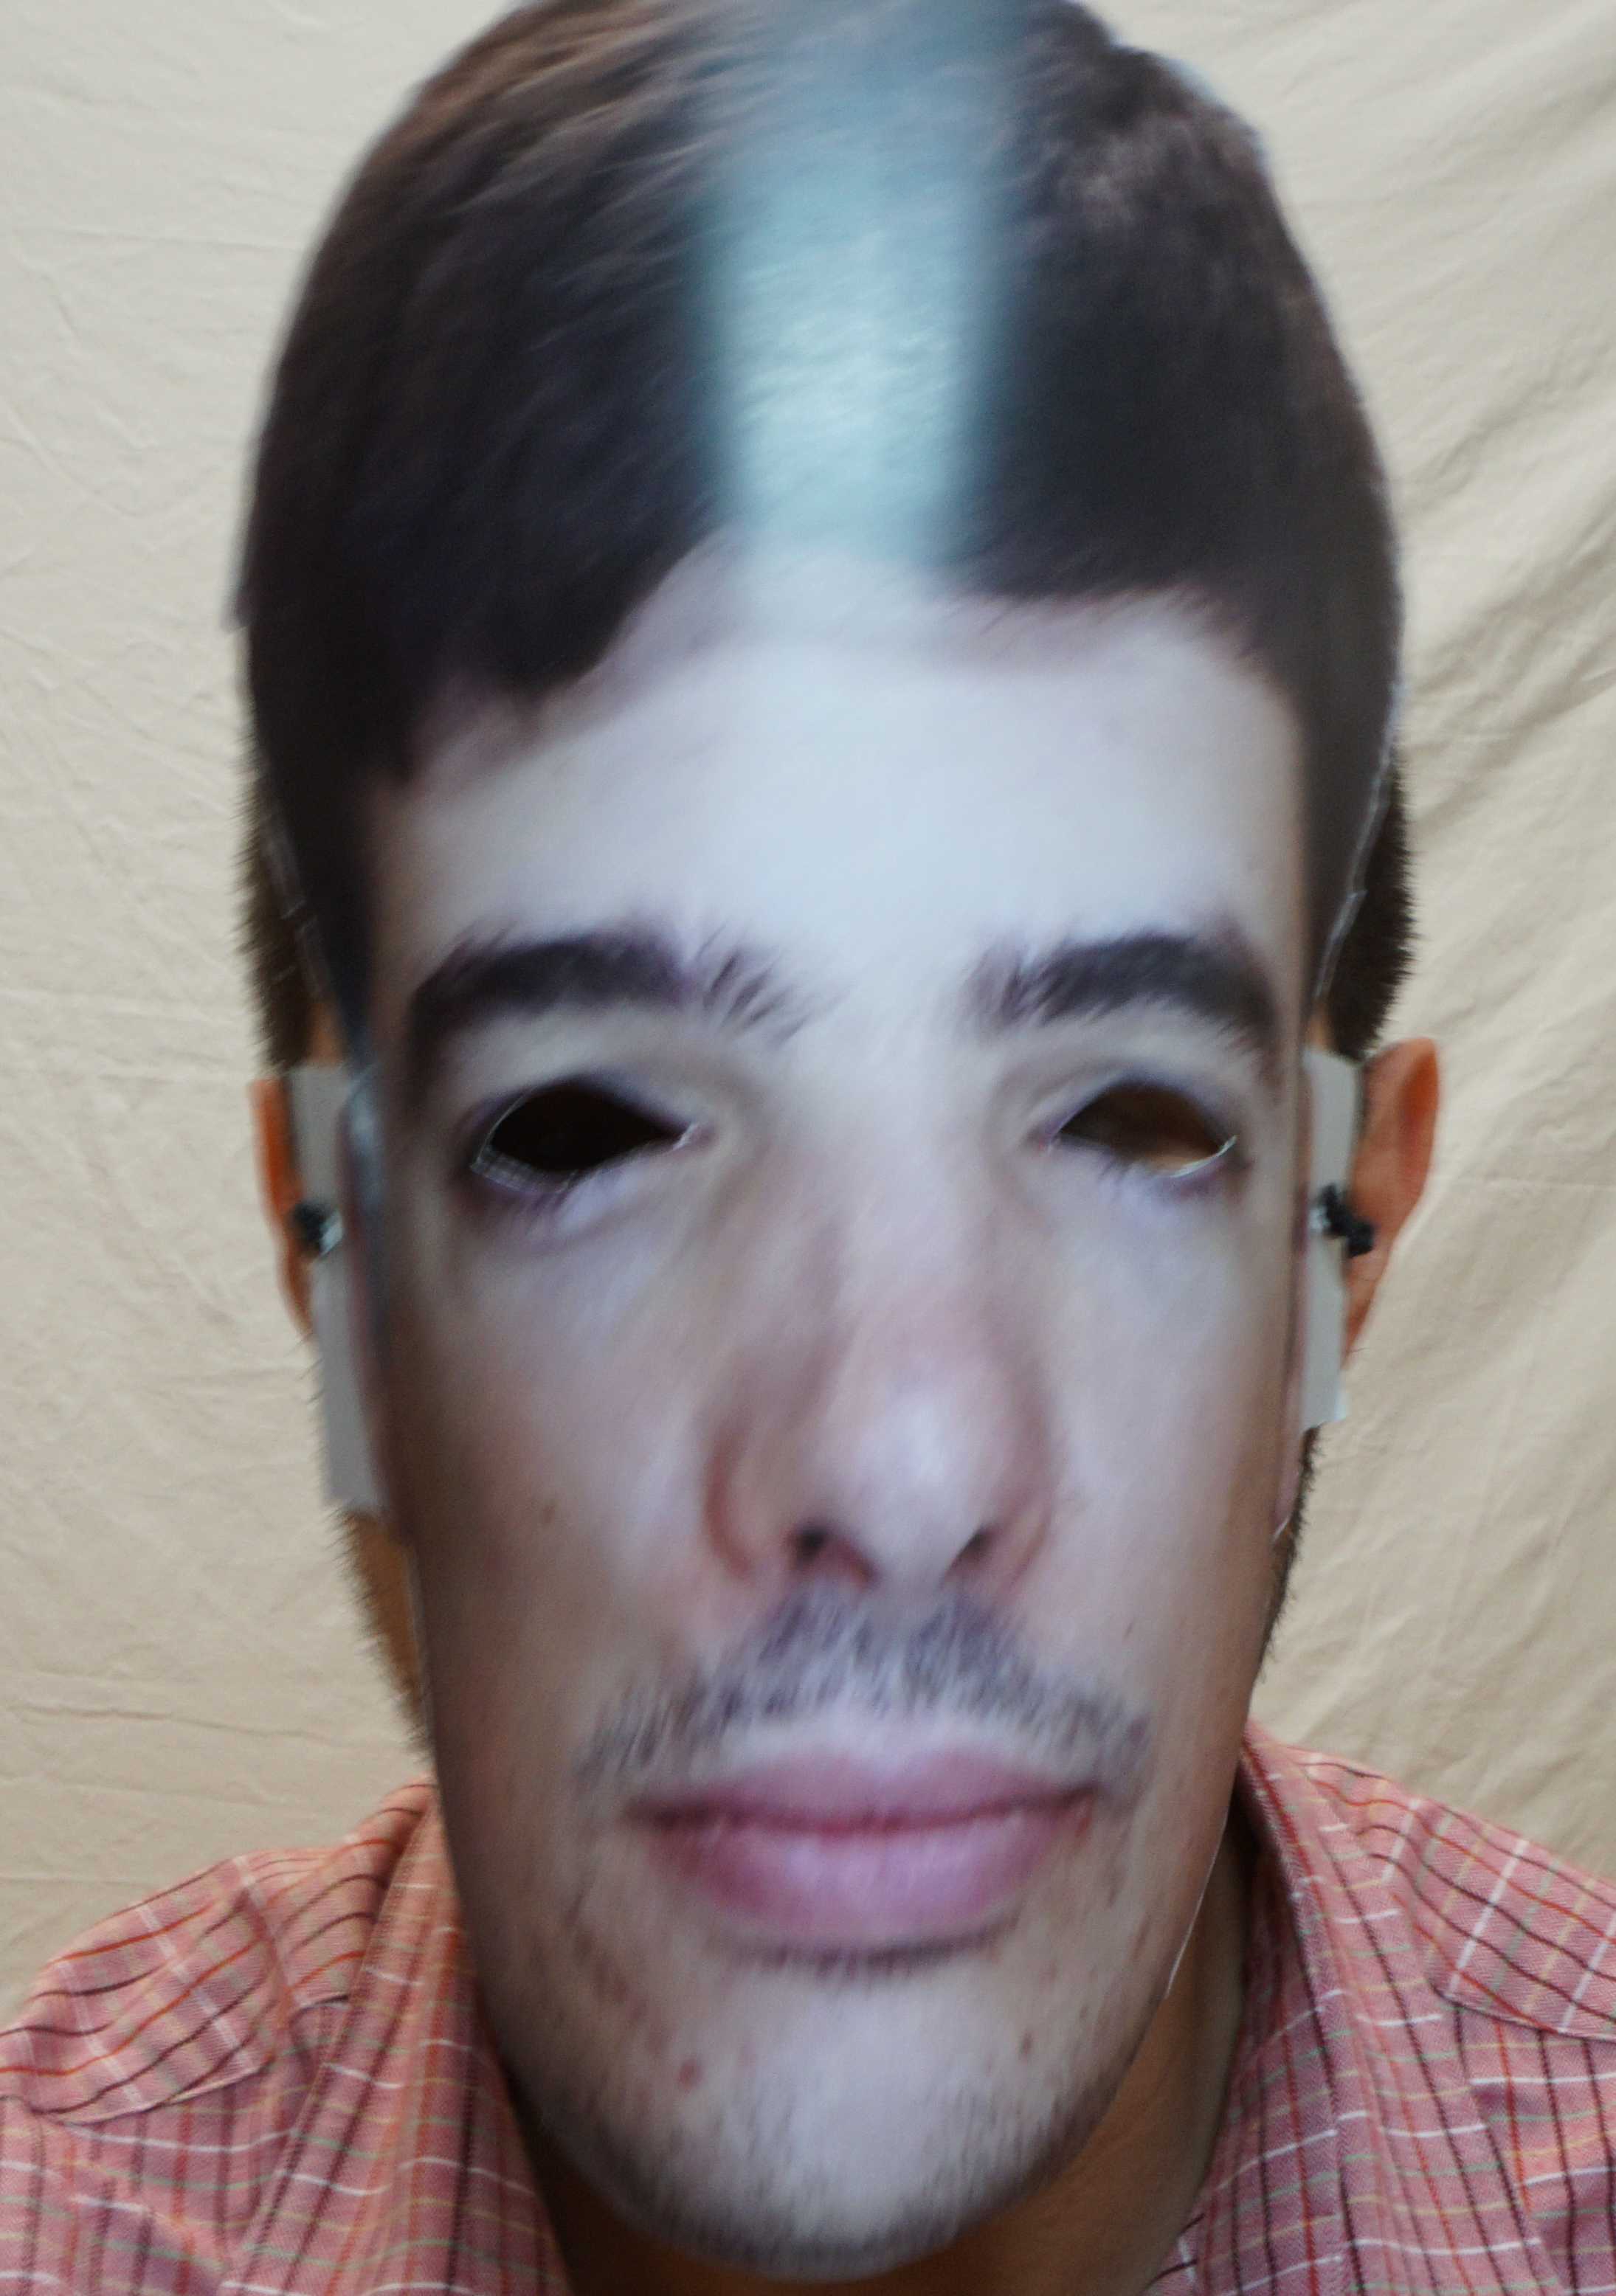
\includegraphics[width=0.18\textwidth]{images_databases/fravrgb/at3-0.JPG} \label{frav_im1-3}}
\subfigure[tablet attack]{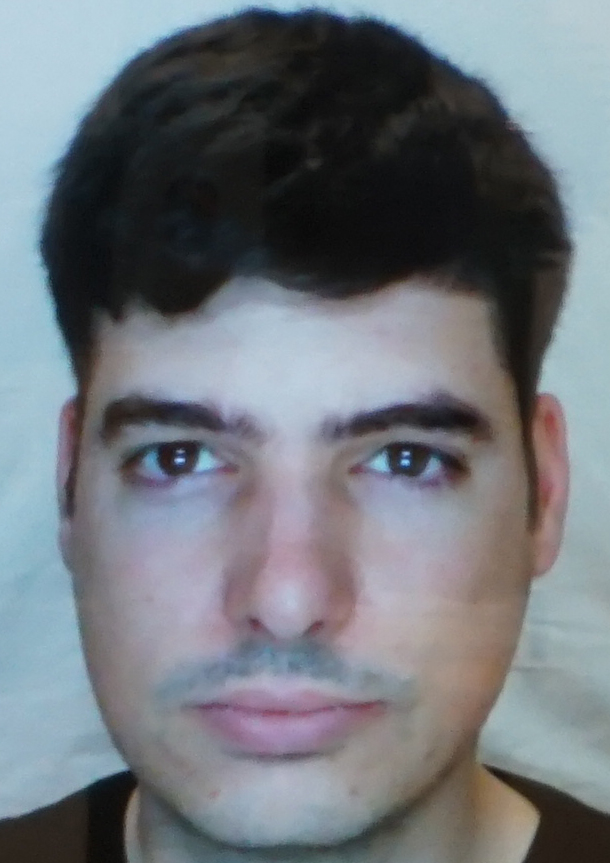
\includegraphics[width=0.18\textwidth]{images_databases/fravrgb/at4-0.JPG} \label{frav_im1-4}}
\subfigure[real user]{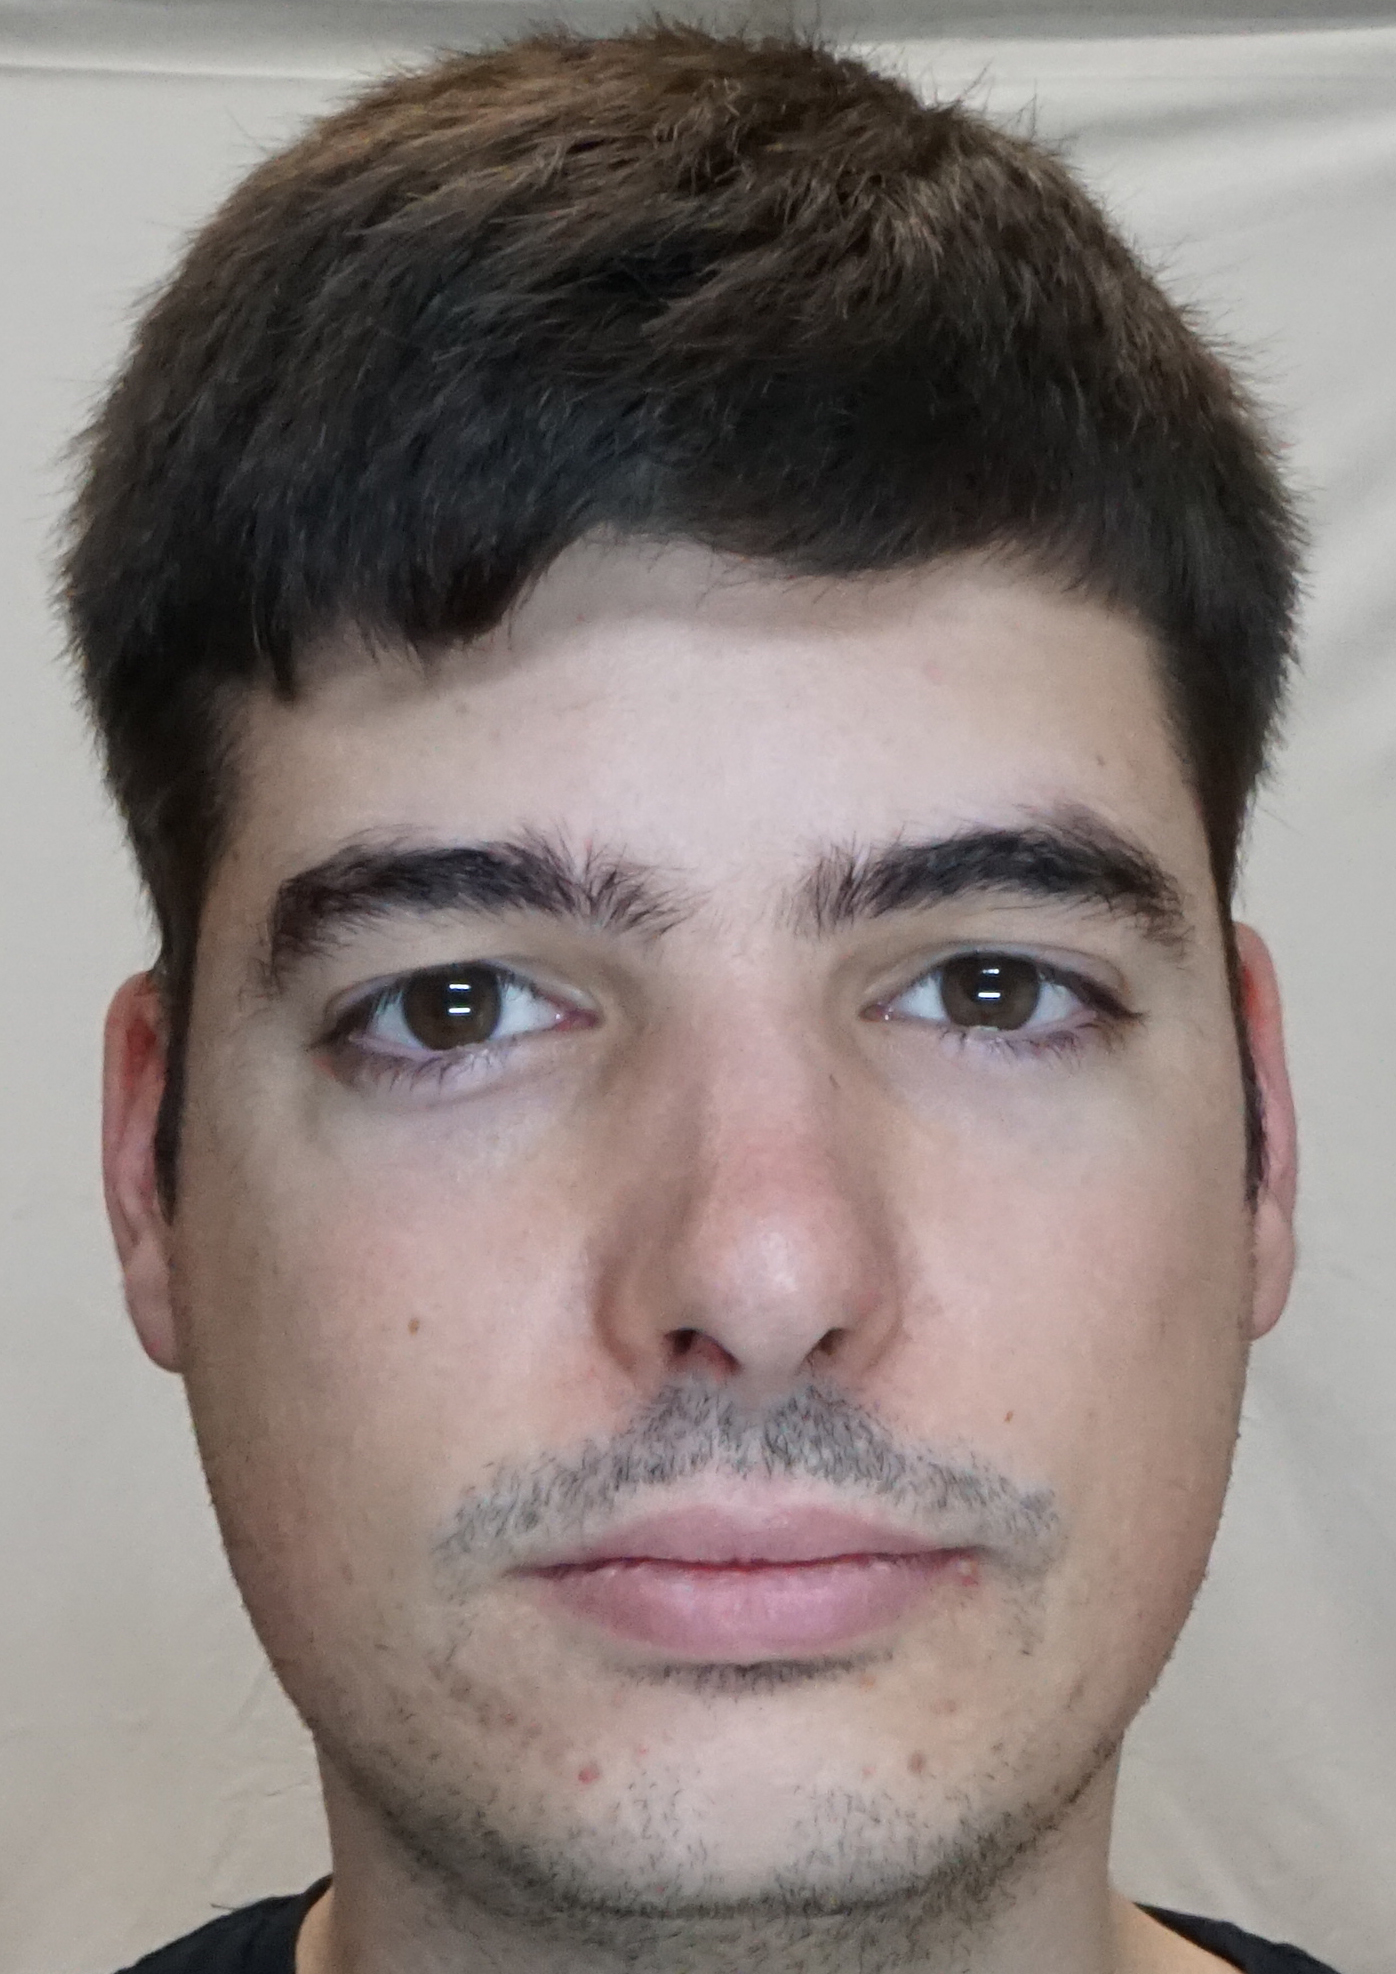
\includegraphics[width=0.18\textwidth]{images_databases/fravrgb/real0.JPG} \label{frav_im1-5}}
\caption{Four attacks and real user from RGB FRAV database.} \label{fig:RGB-frav1}
\end{figure}

\subsubsection{FRAV RGB+NIR database}
This database is smaller that RGB database because not all users have its corresponding NIR image. A representation of RGB database is presented in figure \ref{fig:RGB-frav2}, where each RGB image has its corresponding NIR image.\\

\begin{figure}[htb]
\centering
\subfigure[printed RGB image attack]{ 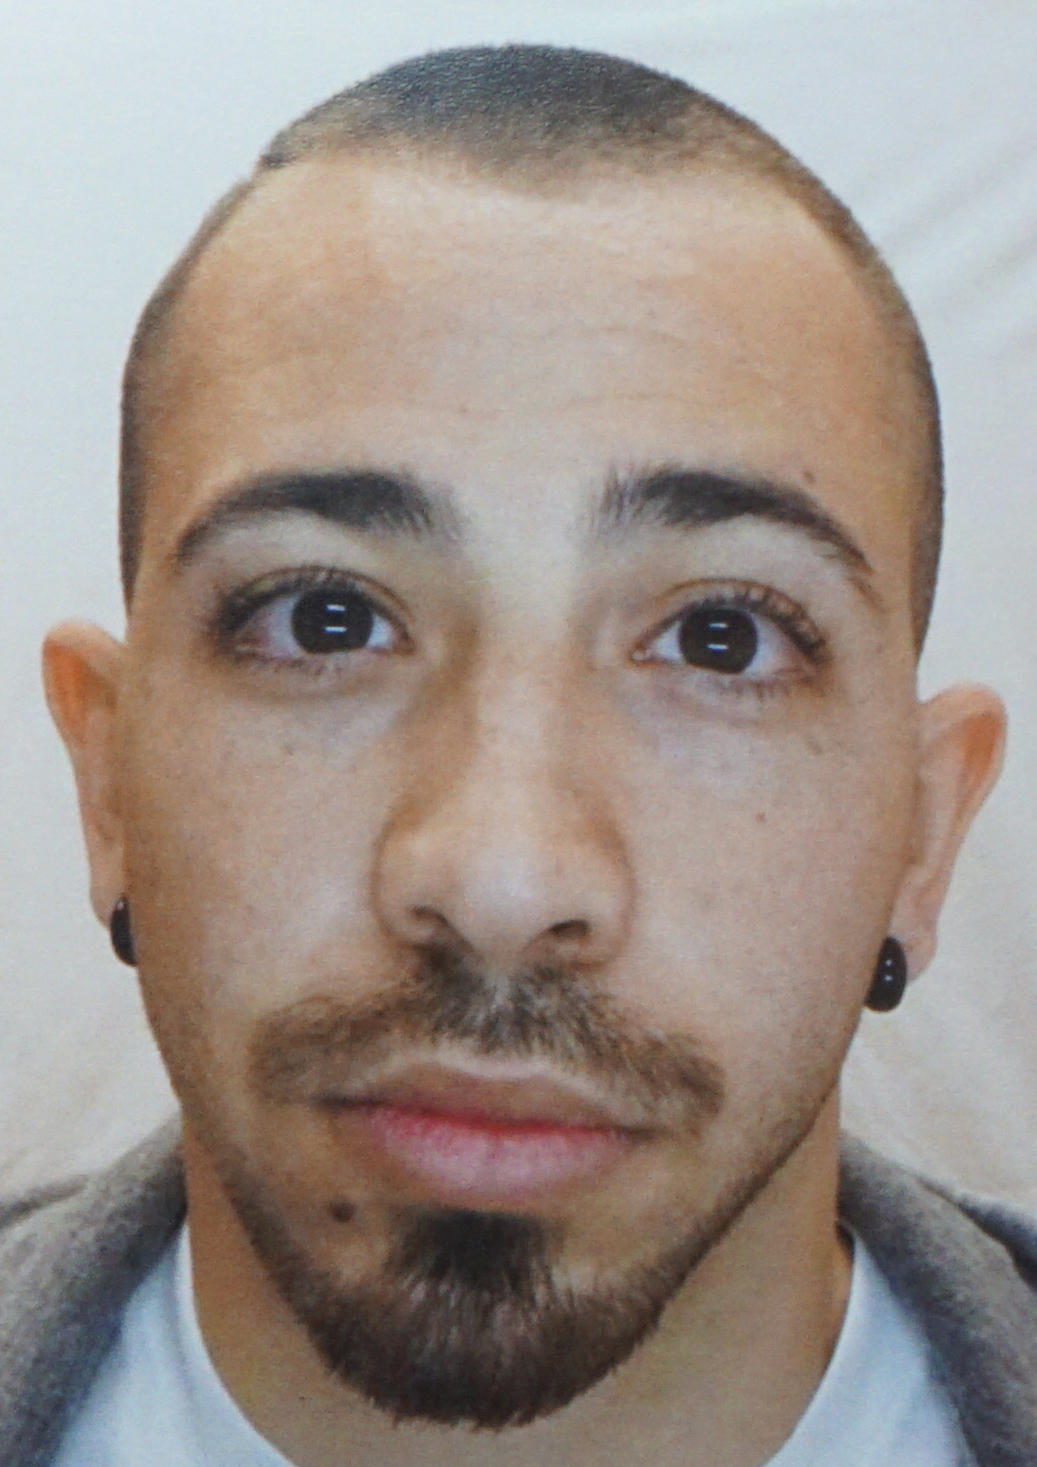
\includegraphics[width=0.18\textwidth]{images_databases/fravrgb/at1-1.JPG} \label{frav_im2-1} }
\subfigure[mask attack RGB]{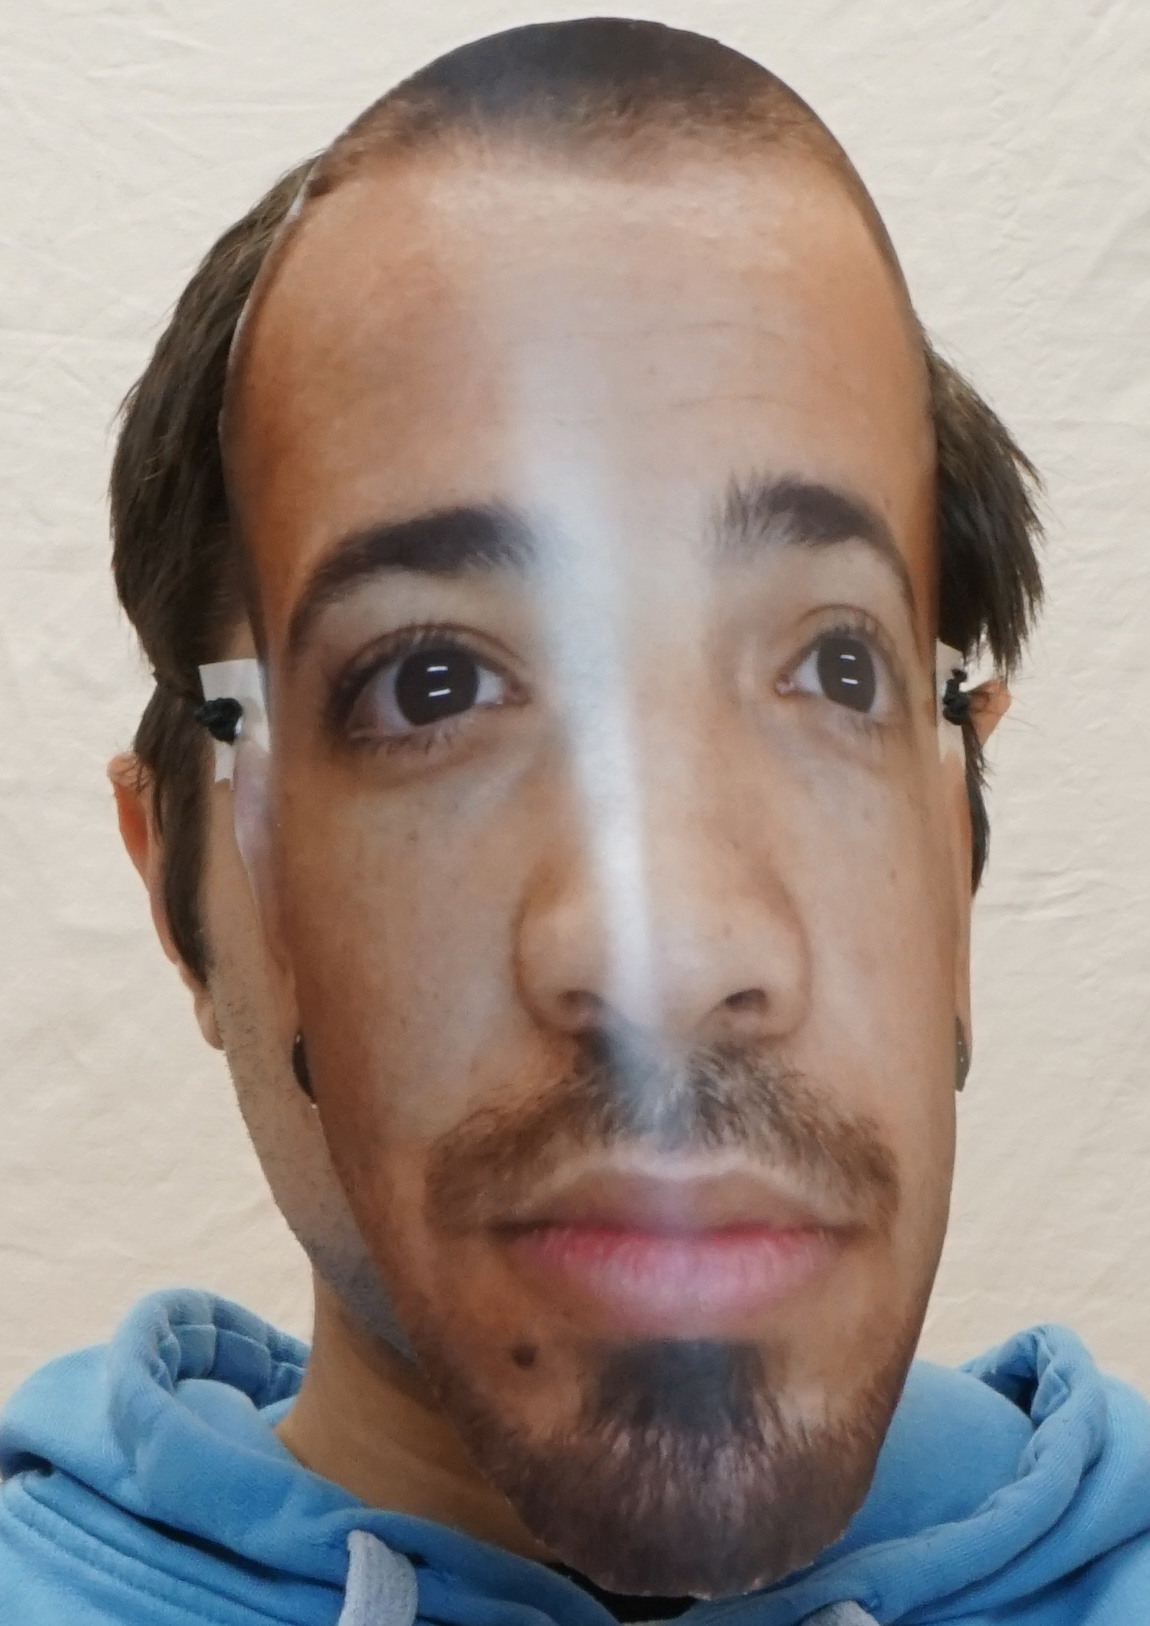
\includegraphics[width=0.18\textwidth]{images_databases/fravrgb/at2-1.JPG} \label{frav_im2-2}}
\subfigure[eye mask attack RGB]{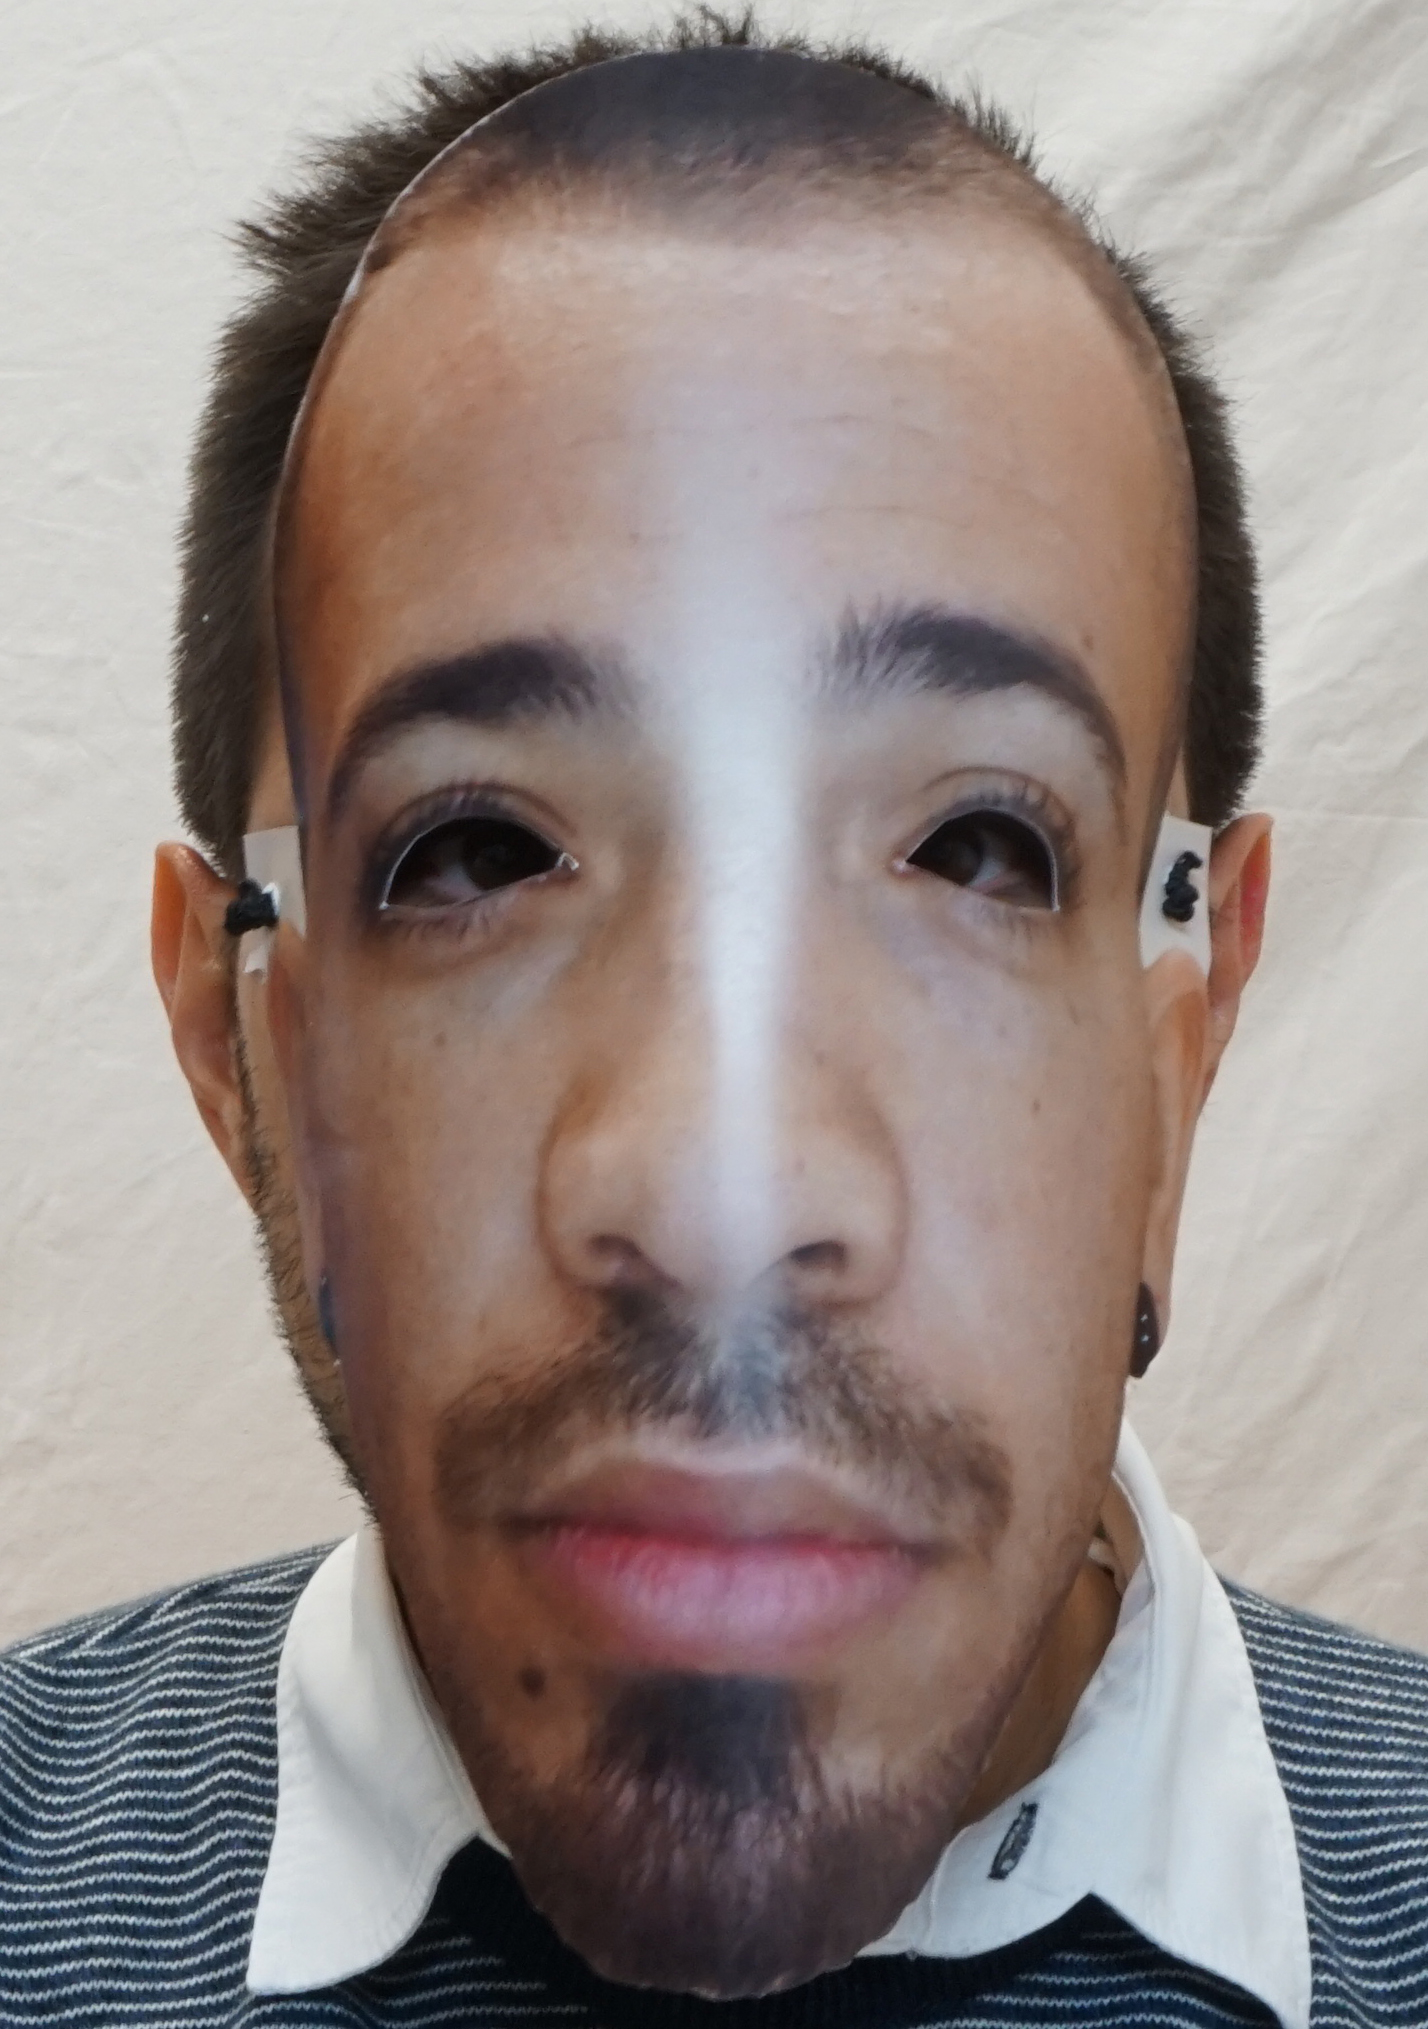
\includegraphics[width=0.18\textwidth]{images_databases/fravrgb/at3-1.JPG} \label{frav_im2-3}}
\subfigure[tablet attack RGB]{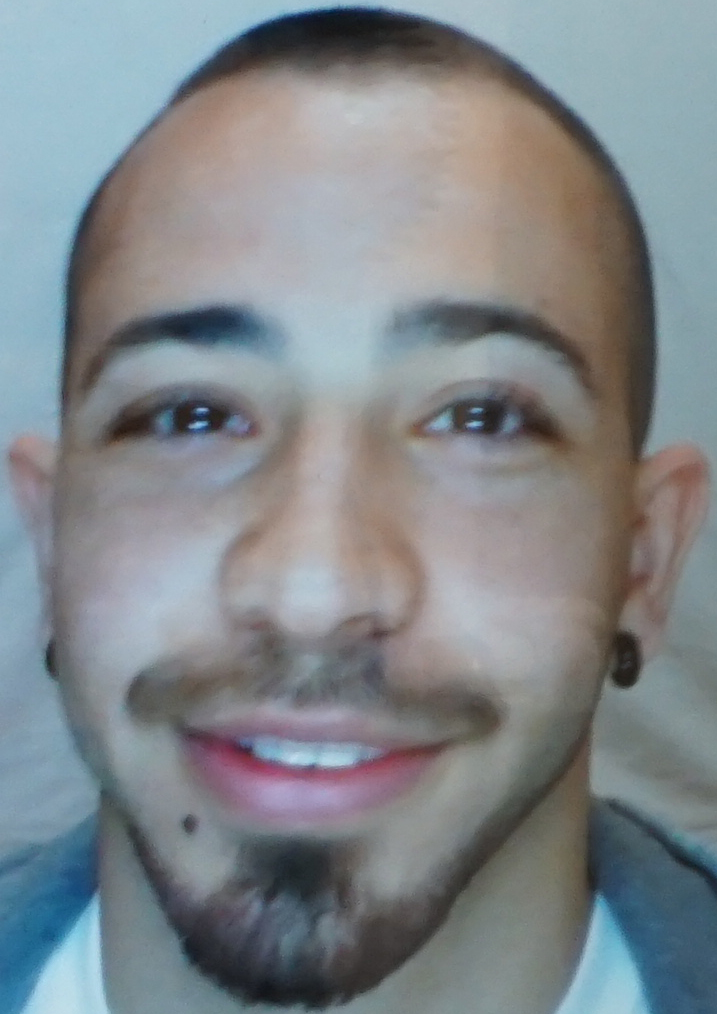
\includegraphics[width=0.18\textwidth]{images_databases/fravrgb/at4-1.JPG} \label{frav_im2-4}}
\subfigure[real user RGB]{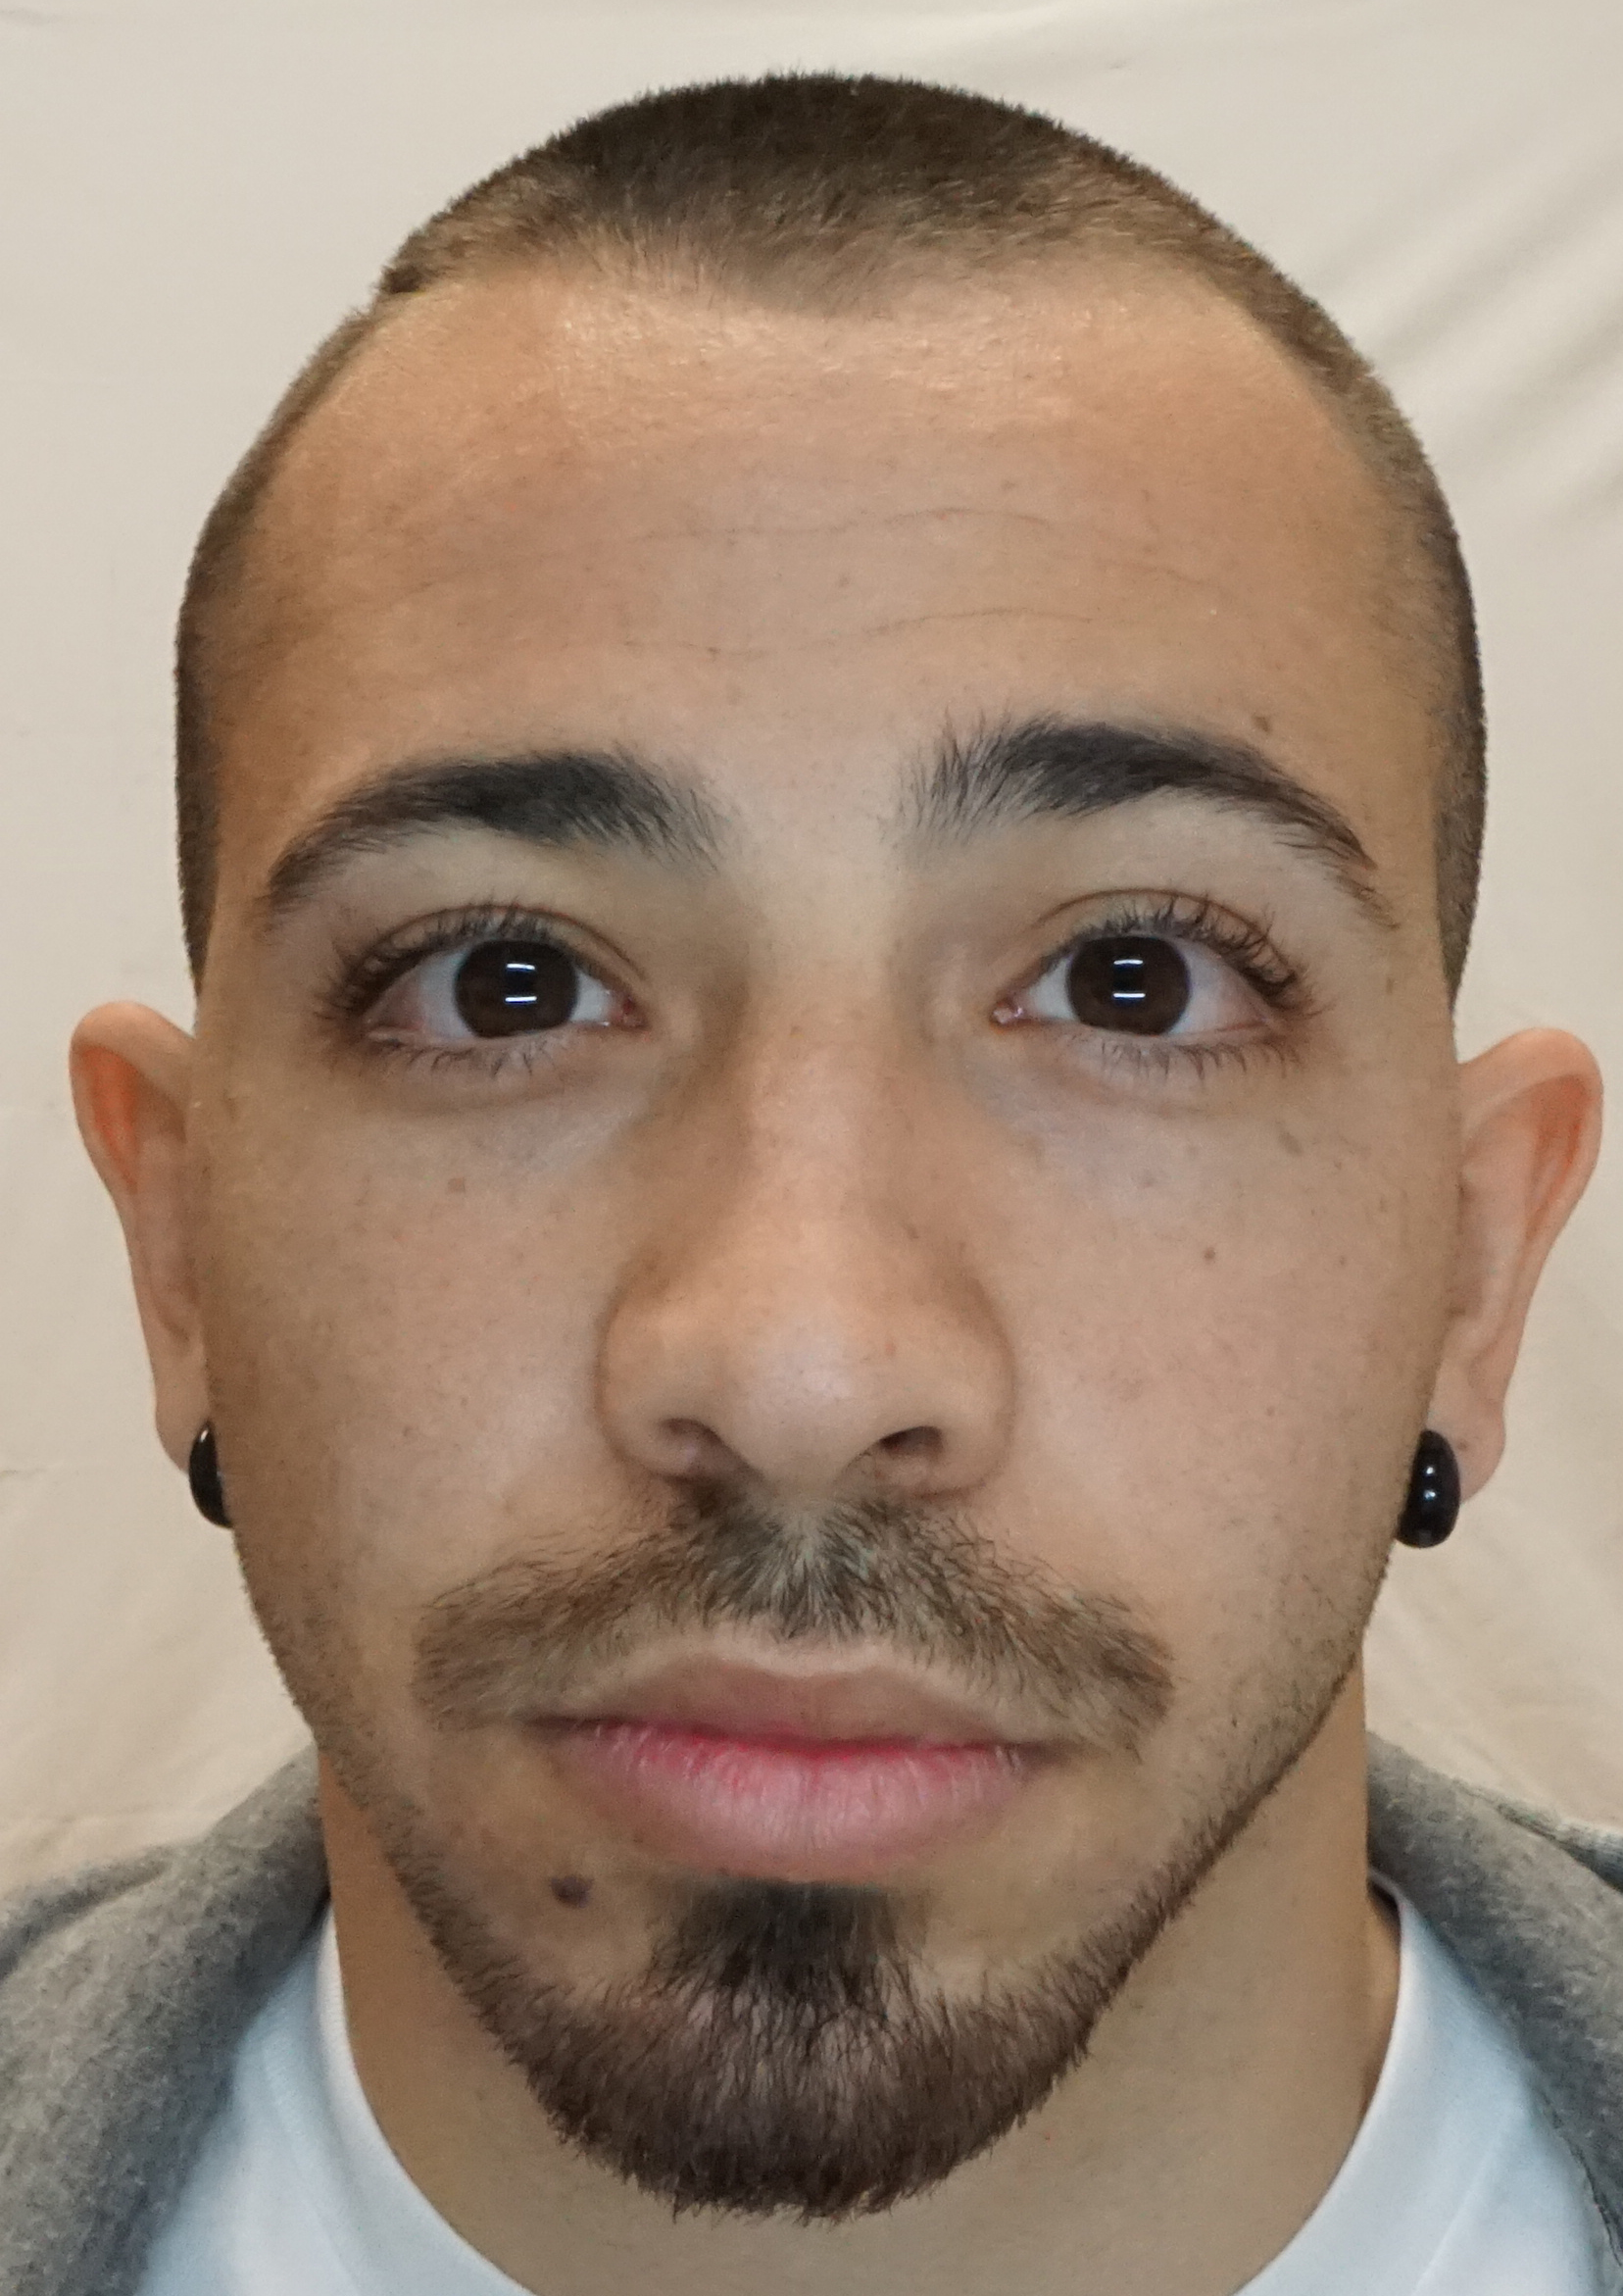
\includegraphics[width=0.18\textwidth]{images_databases/fravrgb/real1.JPG} \label{frav_im2-5}}

\subfigure[printed NIR image attack]{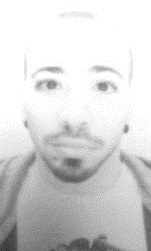
\includegraphics[width=0.18\textwidth]{images_databases/fravnnir/at-1.jpg} \label{frav_im3-1} }
\subfigure[mask attack NIR]{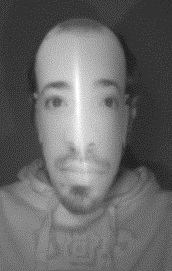
\includegraphics[width=0.18\textwidth]{images_databases/fravnnir/at-2.jpg} \label{frav_im3-2}}
\subfigure[eye mask attack NIR]{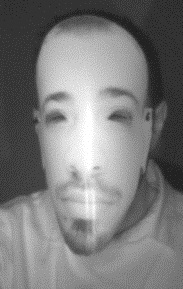
\includegraphics[width=0.18\textwidth]{images_databases/fravnnir/at-3.jpg} \label{frav_im3-3}}
\subfigure[tablet attack NIR]{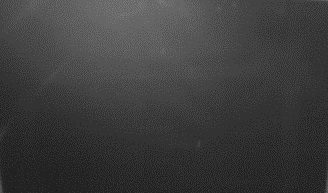
\includegraphics[width=0.18\textwidth]{images_databases/fravnnir/at-4.jpg} \label{frav_im3-4}}
\subfigure[real user NIR]{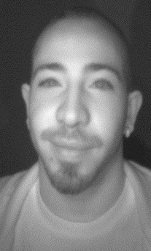
\includegraphics[width=0.18\textwidth]{images_databases/fravnnir/real.jpg} \label{frav_im3-5}}

\caption{Four attacks and real user of RGB and NIR FRAV database.} \label{fig:RGB-frav2}
\end{figure}

When RGB and NIR (figure \ref{fig:RGB-frav2})images are used at the same time, two different methods, with the finality of using both types of images together, are determined:
\begin{itemize}
\item Adding images in characteristic level: adding the NIR image as another layer to RGB image, so the resultant image have hightxweightx4 dimensions (NIR images has one layer because it is a gray scale image and RGB images has three layers, one per each primary color). The network is feed with the resultant images like other times.
\item Adding images in classification level: after the network training and before feeding the classifier, RGB and NIR databases would be trained separately and its features would be appended as the input of the classifier.
\end{itemize}

To conclude, this database is going to be used in the three different ways: just RGB images, RGB and NIR images added in characteristic level or classification level.\\

When the classes are build, two ways are possible to be done: the first one where real people are one class (positive) and the different attacks are another class (negatives), so two classes have been used; and the second way where each attacks correspond with a class, so five classes (4 attacks and 1 real) have been utilized.\\

\subsection{CASIA dataset}
The CASIA Face Anti-Spoofing database is a database from the Chinese Academy of Sciences Centre for Biometrics and Security Research (CASIA-CBSR) \cite{Casiadatbase}.

CASIA database is formed by real or genuine images of people and three different attacks of the same people:
\begin{itemize}[itemsep=2pt,topsep=8pt,parsep=0pt,partopsep=20pt]
 \item Images of people printed (attack) represented in figure \ref{casia_im1-1}.
 \item Images of people with a mask with the eyes cropped (attack) represented in figure \ref{casia_im2-1}.
 \item Tablet attack represented in figure \ref{casia_im3-1}
\item Images of real users represented in figure \ref{casia_im4-1}.
 \end{itemize}

\begin{figure}[htb]
\centering
\subfigure[printed image attack]{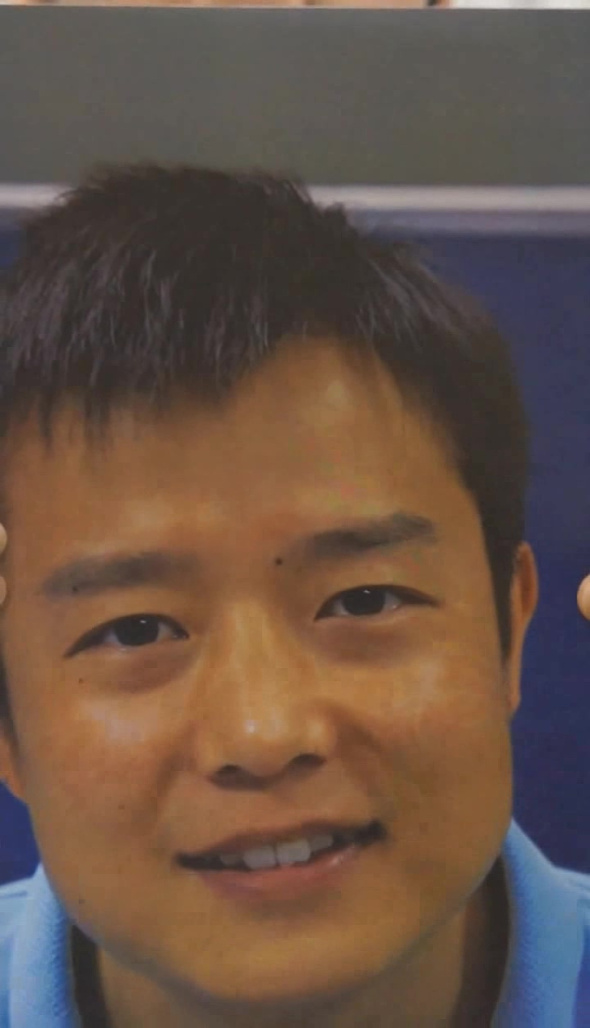
\includegraphics[width=0.2\textwidth]{images_databases/casia/at1-2.jpg} \label{casia_im1-1} }
\subfigure[eye printed image attack]{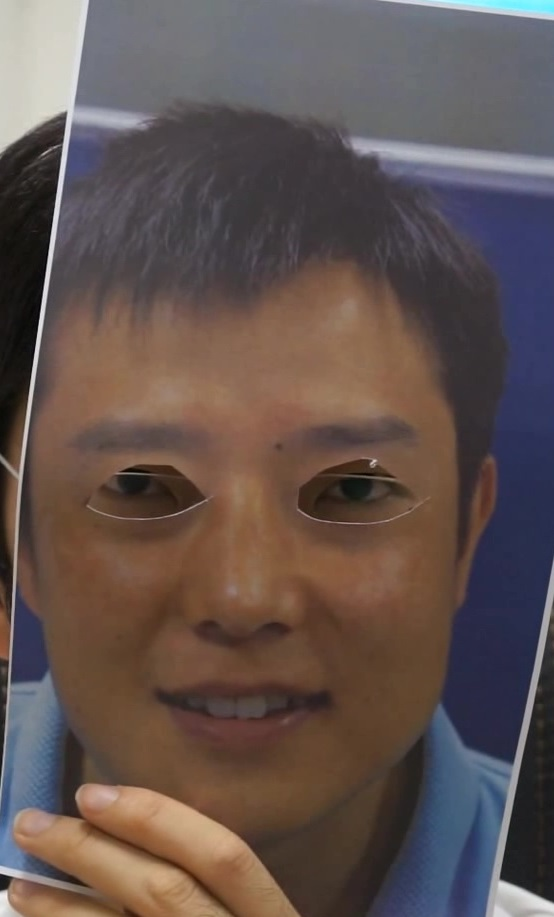
\includegraphics[width=0.2\textwidth]{images_databases/casia/at2-2.jpg} \label{casia_im2-1} }
\subfigure[tablet attack]{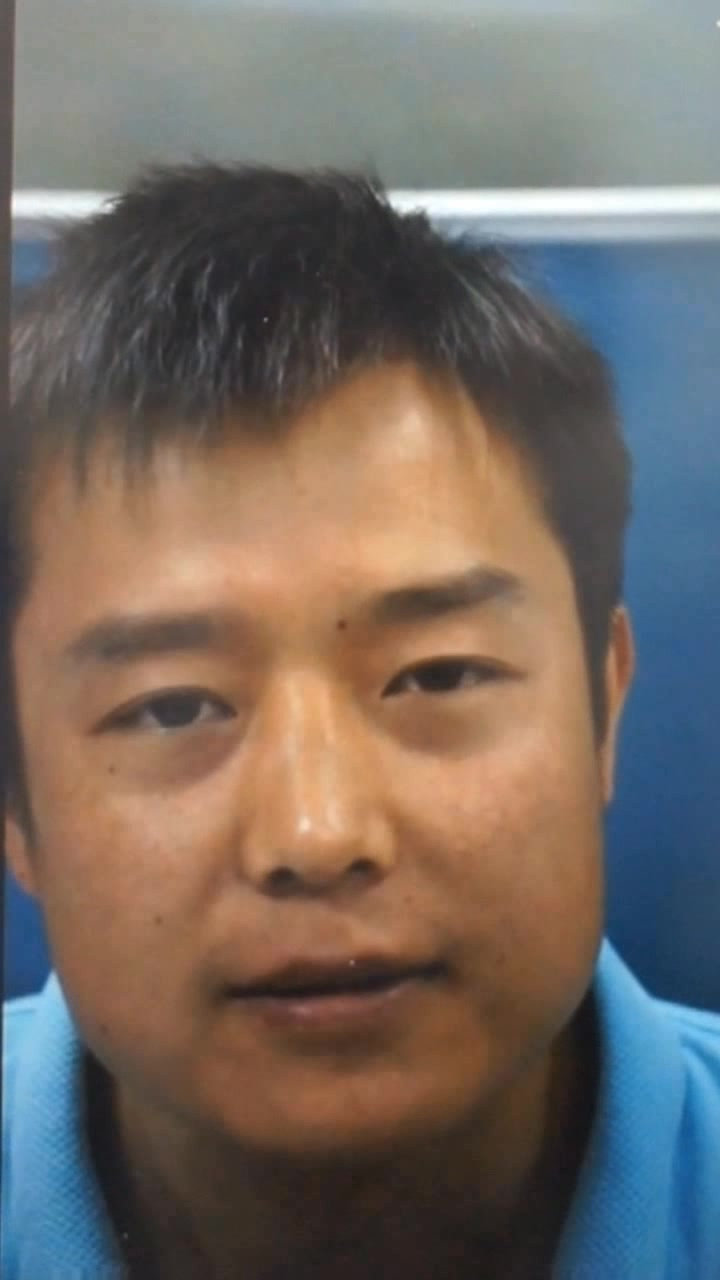
\includegraphics[width=0.2\textwidth]{images_databases/casia/at3-2.jpg} \label{casia_im3-1} }
\subfigure[real user]{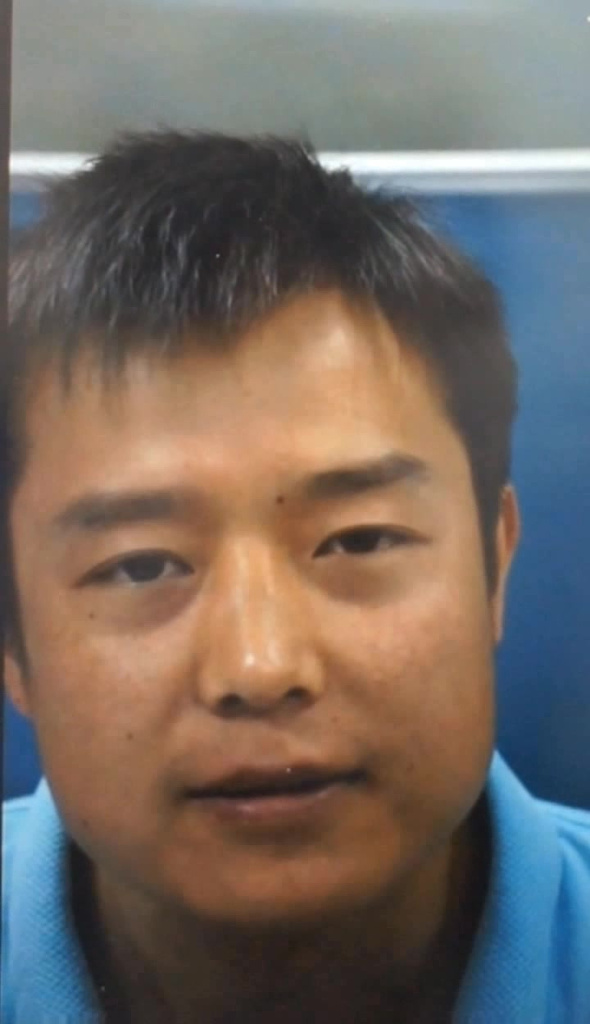
\includegraphics[width=0.2\textwidth]{images_databases/casia/real2.jpg} \label{casia_im4-1} }

\caption{Three attacks and real user from casia database.} \label{fig:casia2}
\end{figure}

Originally, this database is a video database, in which each sample is a different video, but for the experiments developed no videos (entirely or fed directly to the network) have been used. The CASIA database has been used in two different ways:
\begin{itemize} [itemsep=2pt,topsep=8pt,parsep=0pt,partopsep=20pt]
 \item Using a single image per person and class. When this database is used, it is going to be referred as CASIA image database.
 \item Reading three frames per video and saving each frame as a independent image sample. This database is going to be referred as CASIA video database.
\end{itemize}

The characteristics of the CASIA image database are the following ones:
\begin{itemize}[itemsep=2pt,topsep=8pt,parsep=0pt,partopsep=20pt]
\item There are 49 images per user, so there are 196 unique samples.
\item Samples do not have the same size.
\item Samples are in RGB space.
\item The face of the image is centered.
\end{itemize}

The characteristics of the CASIA video database are the following ones:
\begin{itemize}[itemsep=2pt,topsep=8pt,parsep=0pt,partopsep=20pt]
\item There are 8 videos per person (two videos for real user, and two per each attack).
\item There are two videos because one is filmed horizontally and the other vertically, one filmed with a smartphone and the other with the frontal camera of a laptop.
\item There are 50 different users, so there are 400 different videos.
\item For each video 3 frames are read, so there are 1200 unique samples.
\item Samples are in RGB space.
\item Faces are centered in the image and blink expression and movement of people are produced.
\end{itemize}

At the time of assigning a class, it could be done using two classes, the positive class to the real users and the negative class to the attacks; If each attack is assigned to a independent class, it would be four different classes, the real user class and three attack classes.\\

%\begin{figure}[htb]
%\centering
%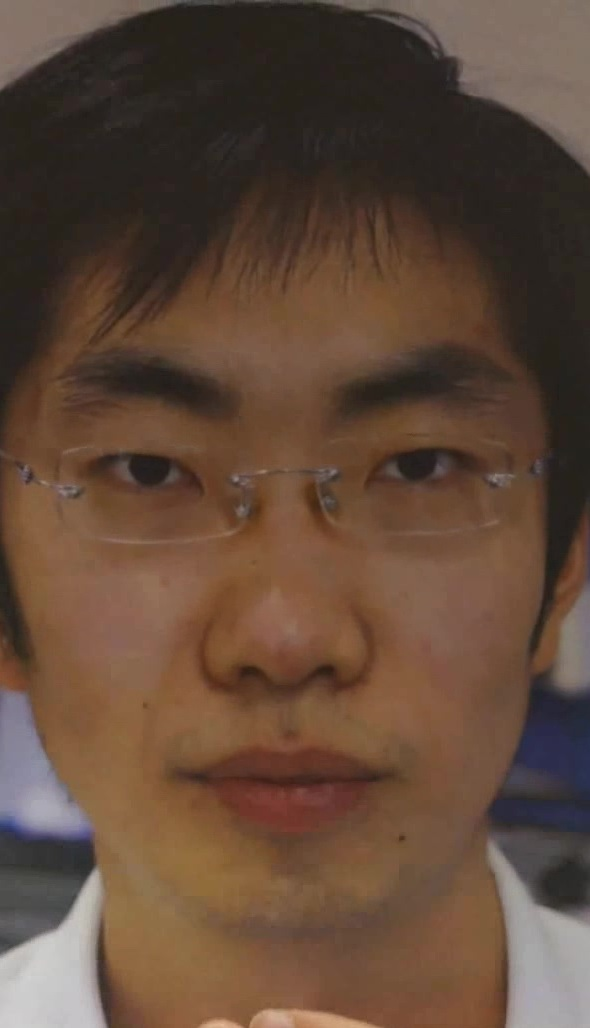
\includegraphics[width=0.2\textwidth]{images_databases/casia/at1-1.jpg}
%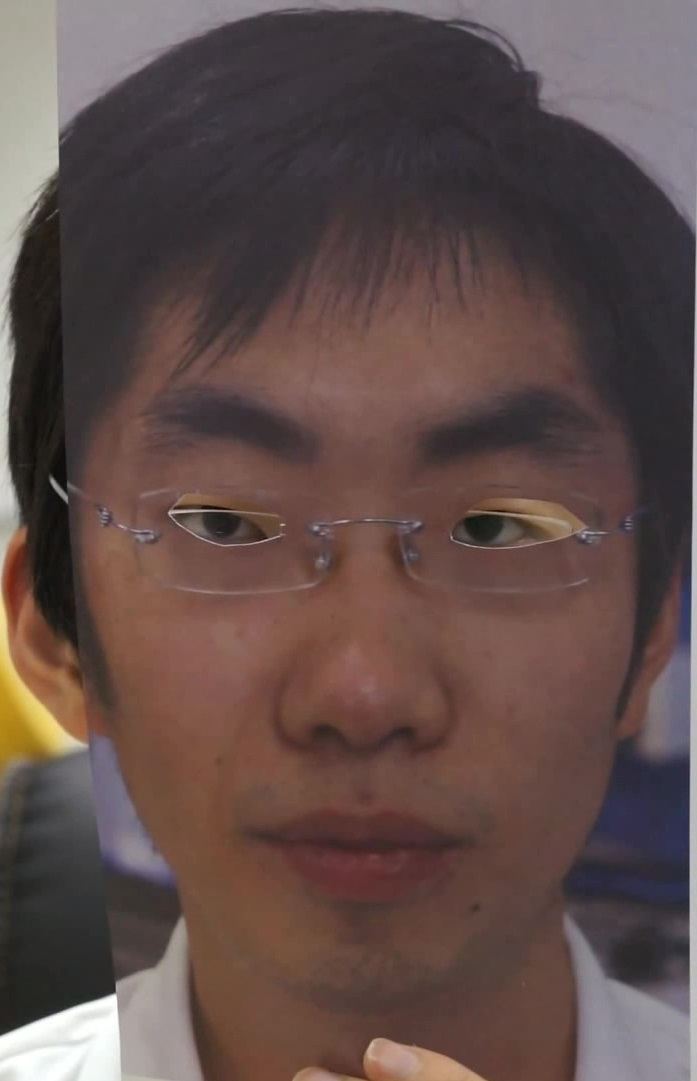
\includegraphics[width=0.2\textwidth]{images_databases/casia/at2-1.jpg}
%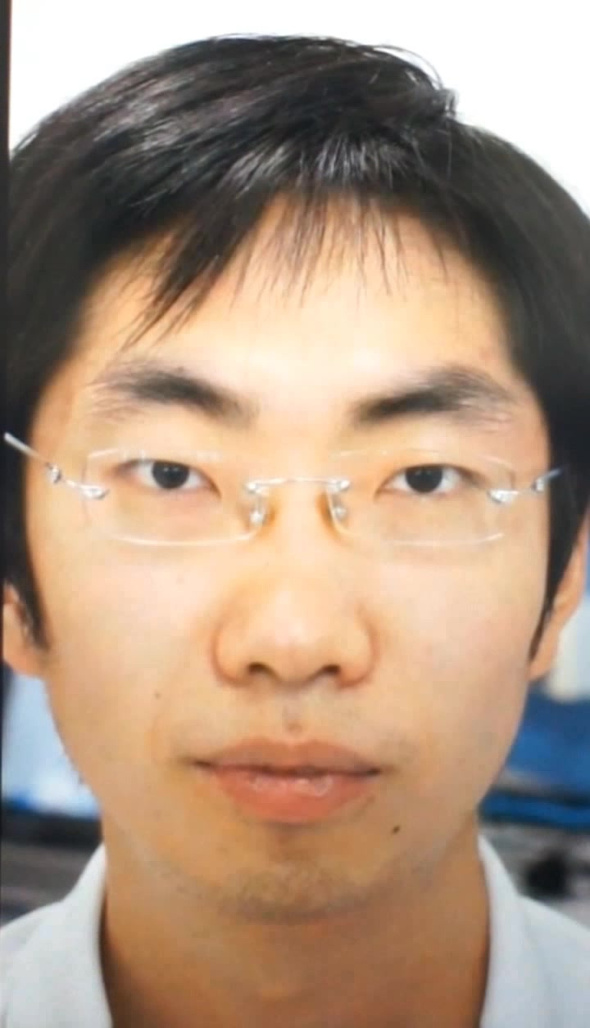
\includegraphics[width=0.2\textwidth]{images_databases/casia/at3-1.jpg}
%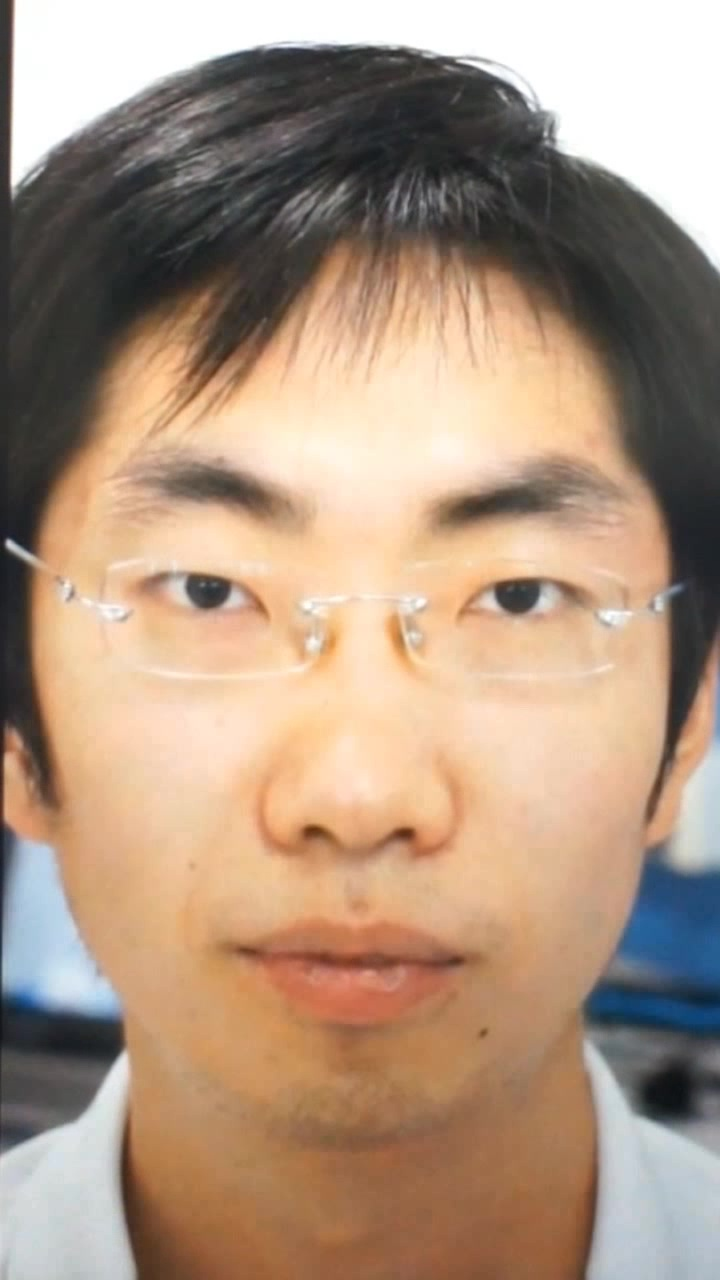
\includegraphics[width=0.2\textwidth]{images_databases/casia/real1.jpg}

%\caption{Three attacks and real user from casia database } \label{fig:casia1}
%\end{figure}

This database has been used in different articles \cite{yangLL14,Spoofing_survey,MSUdatabse,LSTM-CNN}, it is a very utilized databased for face biometrics.\\

\subsection{MSU-MFSD database}
The MSU Mobile Face Spoofing Database (MSU-MFSD) is a video face anti-spoofing database \cite{MSUdatabse}.\\

In figure \ref{fig:mfsd} are represented the three attacks and a real user which forms this database:
\begin{itemize}[itemsep=2pt,topsep=8pt,parsep=0pt,partopsep=20pt]
\item Printed photo attack represented in figure \ref{mfsd_im1-1}.
\item Tablet (iPad Air) attack where a video is Replayed represented in figure \ref{mfsd_im1-1}.
\item Smartphone (iPhone 5s) attack represented in figure \ref{mfsd_im1-1}.
\item Real user represented in figure \ref{mfsd_im1-1}.
\end{itemize}

\begin{figure}[htb]
\centering
\subfigure[printed image attack]{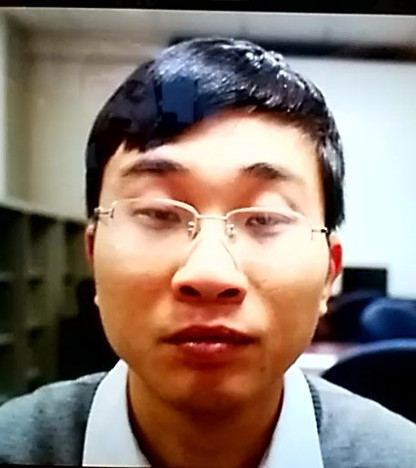
\includegraphics[width=0.2\textwidth]{images_databases/MFSD/at1-1.jpg} \label{mfsd_im1-1} }
\subfigure[tablet attack]{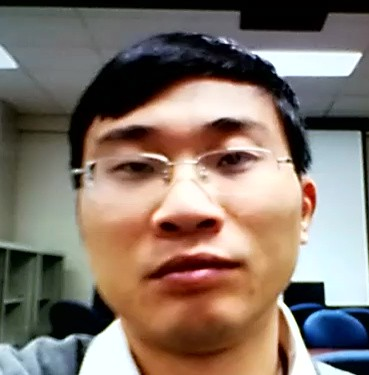
\includegraphics[width=0.2\textwidth]{images_databases/MFSD/at2-1.jpg} \label{mfsd_im2-1} }
\subfigure[smartphone attack]{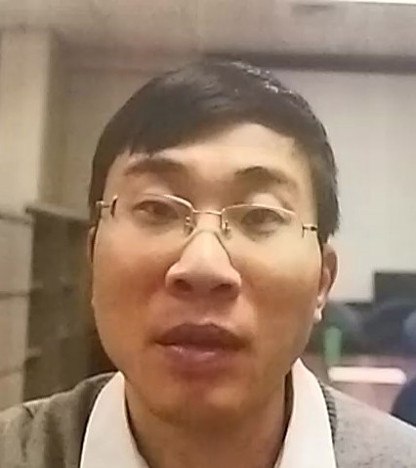
\includegraphics[width=0.2\textwidth]{images_databases/MFSD/at3-1.jpg} \label{mfsd_im3-1} }
\subfigure[real user]{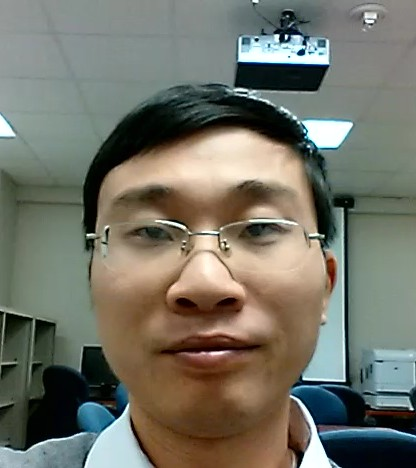
\includegraphics[width=0.2\textwidth]{images_databases/MFSD/1.jpg} \label{mfsd_im4-1} }

\caption{Three attacks and  real user from a person of MFSD database.} \label{fig:mfsd}
\end{figure}

Originally, the database is a video database, but only one frame per user and class is used. The characteristics of the database are the following ones:
\begin{itemize}[itemsep=2pt,topsep=8pt,parsep=0pt,partopsep=20pt]
\item There are 35 images per attack or genuine user. There are 140 unique samples.
\item Images are in RGB space.
\item Faces are centred in images.
\item The size of each image are not equal. Approximately images are 300 pixel heigh and 335 pixel width.
\item Images have been acquired with a Macbook Air laptop and a Google Nexus4 smartphone.
\end{itemize}

%\begin{figure}[htb]
%\centering
%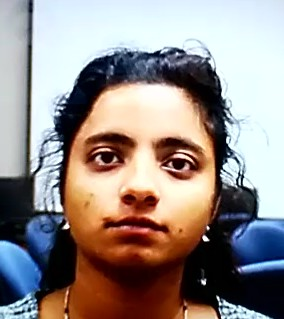
\includegraphics[width=0.2\textwidth]{images_databases/MFSD/at1-2.jpg}
%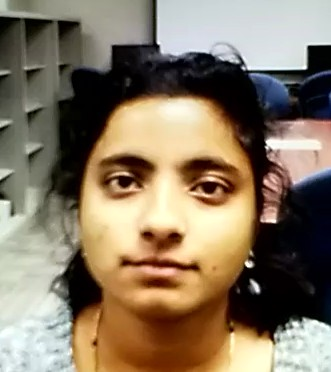
\includegraphics[width=0.2\textwidth]{images_databases/MFSD/at2-2.jpg}
%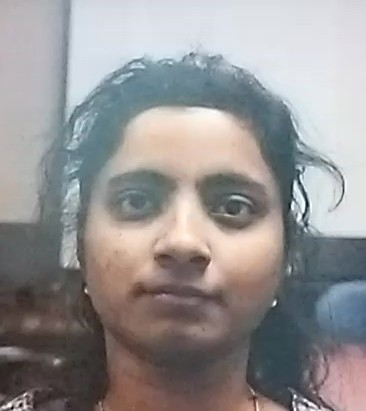
\includegraphics[width=0.2\textwidth]{images_databases/MFSD/at3-2.jpg}
%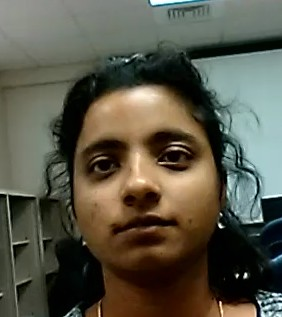
\includegraphics[width=0.2\textwidth]{images_databases/MFSD/2.jpg}
%\caption{Three attacks and real user from a user of MFSD database } \label{fig:mfsd2}
%\end{figure}
